\part{Lecture 10: Value-Based Control with Function Approximation}
\title[RL Lecture 10]{Lecture 10: Value-Based Control \\with Function Approximation}  
\date{}  
\frame{\titlepage} 

%%%%%%%%%%%%%%%%%%%%%%%%%%%%%%%%%%%%%%%%%%%%%%%%%%%%%%%%%%%%%
%% Preface %%
%%%%%%%%%%%%%%%%%%%%%%%%%%%%%%%%%%%%%%%%%%%%%%%%%%%%%%%%%%%%%
\frame{\frametitle{Preface}
Problem space: it is further assumed that
\begin{itemize}
	\item the states $\bm{x}$ are (quasi-)continuous and
	\item the actions $u$ are discrete.
\end{itemize}\pause
\vspace{0.5cm}
Today's focus:
\begin{itemize}
	\item \hl{valued-based control} tasks, i.e., transferring the established tabular methods to work with function approximation.
	\item Hence, we need to extend the previous prediction methods to action values
\end{itemize}
\begin{equation}
			\hat{q}(\bm{x}, u, \bm{w}) \approx q_\pi(\bm{x}, u) .
\end{equation}\pause
\begin{itemize}
	\item And apply the well-known generalized policy iteration scheme (GPI) to find optimal actions:
\end{itemize}
\begin{equation}
			\hat{q}(\bm{x}, u, \bm{w}) \approx q^*(\bm{x}, u) .
\end{equation}
}

%%%%%%%%%%%%%%%%%%%%%%%%%%%%%%%%%%%%%%%%%%%%%%%%%%%%%%%%%%%%%
%% Types of Action-Value Function Approximation %%
%%%%%%%%%%%%%%%%%%%%%%%%%%%%%%%%%%%%%%%%%%%%%%%%%%%%%%%%%%%%%
\frame{\frametitle{Types of action-value function approximation}
\begin{figure}
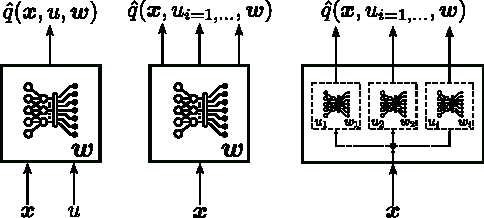
\includegraphics[width=9.5cm]{fig/lec10/Model_types_action_value.pdf}
\label{fig:Model_types_action_value}
\caption{Possible function approximation settings for discrete actions}
\end{figure}
\begin{itemize}
	\item Left: one function with both states and actions as input
	\item Middle: one function with $i=1,2,\ldots$ outputs covering the action space (e.g., ANN with appropriate output layer)
	\item Right: multiple (sub-)functions one for each possible action $u_i$ (e.g., multitude of linear approximators in small action spaces)
\end{itemize}
}

%%%%%%%%%%%%%%%%%%%%%%%%%%%%%%%%%%%%%%%%%%%%%%%%%%%%%%%%%%%%%
%% Feature Engineering %%
%%%%%%%%%%%%%%%%%%%%%%%%%%%%%%%%%%%%%%%%%%%%%%%%%%%%%%%%%%%%%
\frame{\frametitle{Feature engineering}
\begin{itemize}
	\item Also for action-value estimation a proper feature engineering (FE) is of vital importance.
	\item Compared to the state-value prediction, the action becomes part of the FE processing: 
\begin{equation}
	\hat{q}(\bm{x}, u, \bm{w}) = \hat{q}\left(\bm{f}\left(\bm{x}, u\right), \bm{w}\right) .
\end{equation}
	\item Above, $\bm{f}(\bm{x},u)\in\mathbb{R}^\kappa$ is the FE function.\pause
	\item \hl{For sake of notation simplicity we write $\hat{q}(\bm{x}, u, \bm{w})$ and understand that FE has already been considered (i.e., is a part of $\hat{q}$).}
\end{itemize}
}



%%%%%%%%%%%%%%%%%%%%%%%%%%%%%%%%%%%%%%%%%%%%%%%%%%%%%%%%%%%%%%%%%%
\section{On-policy control with (semi-)gradients} 
%%%%%%%%%%%%%%%%%%%%%%%%%%%%%%%%%%%%%%%%%%%%%%%%%%%%%%%%%%%%%%%%%%
\begin{frame}
\frametitle{Table of contents}
\tableofcontents
\end{frame}

%%%%%%%%%%%%%%%%%%%%%%%%%%%%%%%%%%%%%%%%%%%%%%%%%%%%%%%%%%%%%
%% Gradient-Based Action-Value Learning %%
%%%%%%%%%%%%%%%%%%%%%%%%%%%%%%%%%%%%%%%%%%%%%%%%%%%%%%%%%%%%%
\frame{\frametitle{Gradient-based action-value learning}

\begin{itemize}
	\item Transferring the objective \eqref{eq:VE_J} from on-policy prediction to control yields:
\begin{equation}
	J(\bm{w})= \sum_k \left[q_{\pi}(\bm{x}_k, u_k) - \hat{q}(\bm{x}_k, u_k, \bm{w})\right]^2 .
\label{eq:VE_J_action}
\end{equation}\pause
\item Analogous, the (semi-)gradient-based parameter update from \eqref{eq:gradient_param_value} is also applied to action values:
 \begin{equation}
	 \bm{w}_{k+1} = \bm{w}_{k} + \alpha\left[q_\pi(\bm{x}_k, u_k) - \hat{q}(\bm{x}_k, u_k, \bm{w}_k)\right]\nabla_{\bm{w}} \hat{q}(\bm{x}_k, u_k, \bm{w}_k) .
	\label{eq:gradient_param_value_action}
 \end{equation}\pause
\item Depending on the control approach, the true target $q_\pi(\bm{x}_k, u_k)$ is approximated by:
\begin{itemize}
	\item Monte Carlo: full episodic return $q_\pi(\bm{x}_k, u_k) \approx g$,\pause
	\item SARSA: one-step bootstrapped estimate $q_\pi(\bm{x}_k, u_k) \approx r_{k+1}+\gamma\hat{q}(\bm{x}_{k+1}, u_{k+1}, \bm{w}_k)$,\pause
	\item $n$-step SARSA: $q_\pi(\bm{x}_k, u_k) \approx r_{k+1}+\gamma r_{k+2}+\cdots+\gamma^{n-1} r_{k+n}+\gamma^n\hat{q}(\bm{x}_{k+n}, u_{k+n}, \bm{w}_{k+n-1})$.
\end{itemize}
\end{itemize}
}

%%%%%%%%%%%%%%%%%%%%%%%%%%%%%%%%%%%%%%%%%%%%%%%%%%%%%%%%%%%%%
%% Houston: We have a Problem %%
%%%%%%%%%%%%%%%%%%%%%%%%%%%%%%%%%%%%%%%%%%%%%%%%%%%%%%%%%%%%%
\frame{\frametitle{Houston: we have a problem}
\begin{itemize}
	\item Recall tabular \hl{policy improvement theorem} (\theoref{theo:Policy_improvement}): guarantee to find a globally better or equally good policy in each update step.\pause
	\item With parameter updates \eqref{eq:gradient_param_value_action} generalization applies. 
	\item Hence, when reacting to one specific state-action transition other parts of the state-action space within $\hat{q}$ are affected too. \pause
\end{itemize}
\vspace{0.5cm}
\begin{columns}[t,onlytextwidth]
\begin{column}{0.4\textwidth}
\begin{minipage}[c]{\linewidth}
\begin{figure}
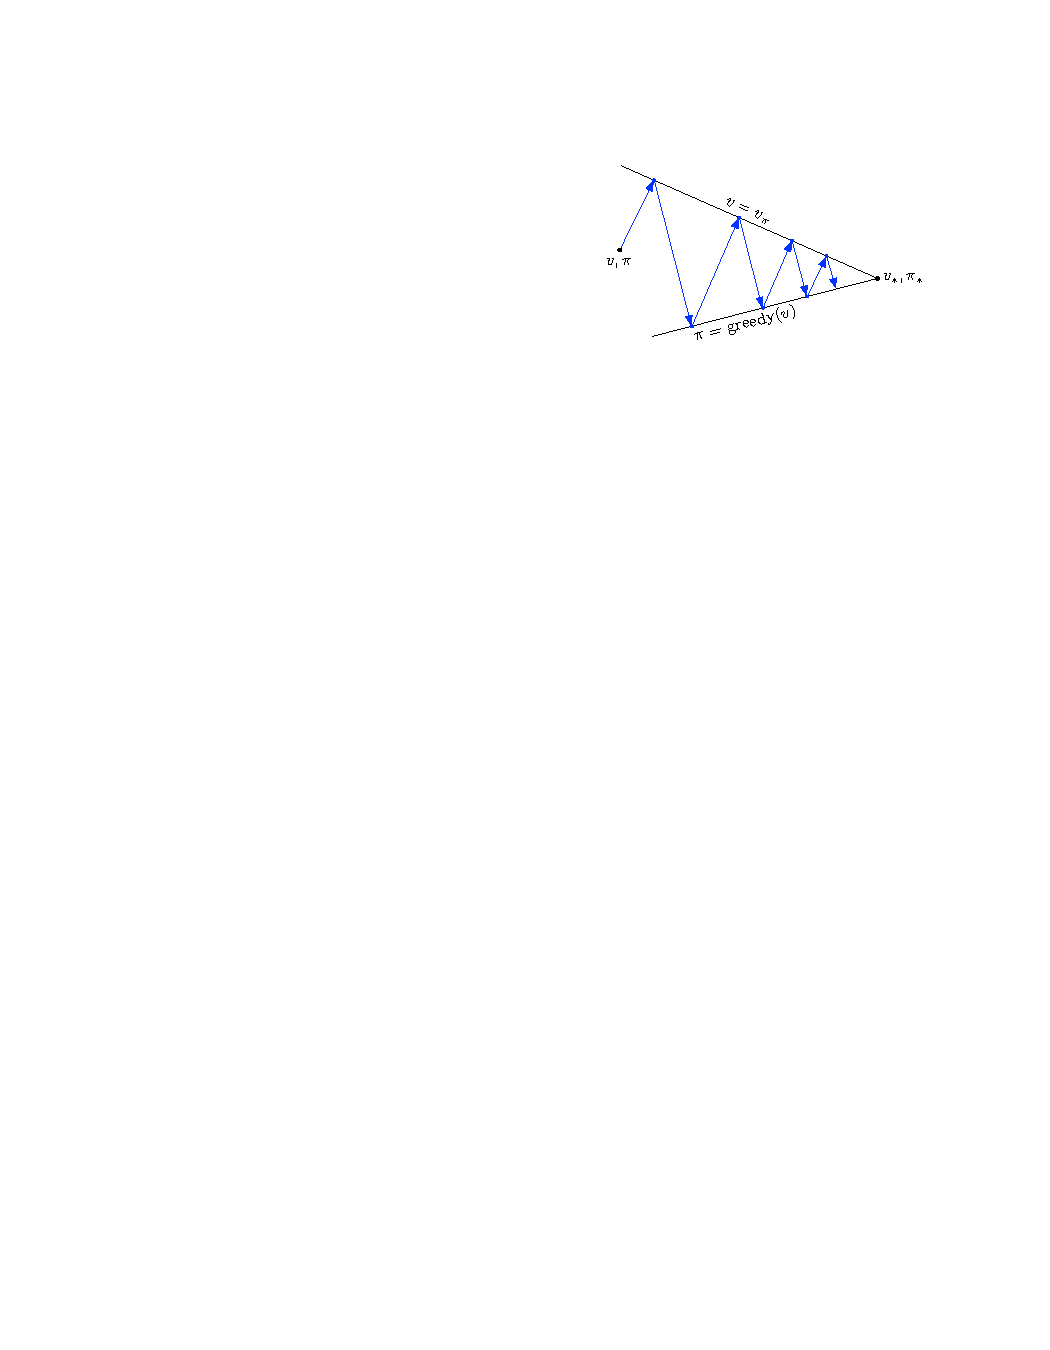
\includegraphics[height=2.5cm]{fig/lec03/GPI_02.pdf}
\caption{GPI}
\end{figure}
\end{minipage}
\end{column}
\hfill
\begin{column}{0.57\textwidth}
\begin{minipage}[c]{\linewidth}
\begin{block}{Loss of policy improvement theorem}
	\begin{itemize}
		\item Is not applicable with function approximation!
		\item We may improve and impair the policy at the same time!
	\end{itemize}
\end{block}
\end{minipage}
\end{column}
\end{columns}

}


%%%%%%%%%%%%%%%%%%%%%%%%%%%%%%%%%%%%%%%%%%%%%%%%%%%%%%%%%%%%%
%% Gradient Monte Carlo On-Policy Control %%
%%%%%%%%%%%%%%%%%%%%%%%%%%%%%%%%%%%%%%%%%%%%%%%%%%%%%%%%%%%%%
\frame{\frametitle{Algorithmic implementation: gradient MC control}
\begin{itemize}
	\item Direct transfer from tabular case to function approximation
	\item Update target becomes the sampled return $q_\pi(\bm{x}_k, u_k)\approx g_k$ 
	\item If operating $\varepsilon$-greedy on $\hat{q}$: baseline policy (given by $\bm{w}_0$) must (successfully) terminate the episode! 
\end{itemize}
\setlength{\algomargin}{0.5em}
\begin{algorithm}[H]
\SetKwInput{Input}{input} 
\SetKwInput{Output}{output}
\SetKwInput{Init}{init}
\SetKwInput{Param}{parameter}
\Input{a differentiable function $\hat{q}:\mathbb{R}^\kappa\times\mathbb{R}^\zeta\rightarrow\mathbb{R}$}
\Input{a policy $\pi$ (only if estimating $q_\pi$)}
\Param{step size $\alpha\in\left\{\mathbb{R}|0<\alpha<1\right\}$, $\varepsilon\in\left\{\mathbb{R}|0<\varepsilon<<1\right\}$}
\Init{parameter vector $\bm{w}\in\mathbb{R}^\zeta$ arbitrarily}
 \For{$j=1,2,\ldots,$ episodes}{
		generate episode following $\pi$ or $\varepsilon$-greedy on $\hat{q}$: $x_{0}, u_{0}, r_{1},\ldots,x_{T}$ \;
		calculate every-visit return $g_k$\;  
		\For{$k=0,1,\ldots, T-1$ time steps}{
			$\bm{w} \leftarrow \bm{w} + \alpha\left[g_k - \hat{q}(\bm{x}_k, u_k,\bm{w})\right]\nabla_{\bm{w}} \hat{q}(\bm{x}_k, u_k, \bm{w})$\; 
		}
	}
\caption{Every-visit gradient MC-based action-value estimation (output: parameter vector $\bm{w}$ for $\hat{q}_\pi$ or $\hat{q}^*$)}
\label{algo:MC_gradient_control}
\end{algorithm}
}

%%%%%%%%%%%%%%%%%%%%%%%%%%%%%%%%%%%%%%%%%%%%%%%%%%%%%%%%%%%%%
%% Semi-Gradient Sarsa %%
%%%%%%%%%%%%%%%%%%%%%%%%%%%%%%%%%%%%%%%%%%%%%%%%%%%%%%%%%%%%%
\frame{\frametitle{Algorithmic implementation: semi-gradient SARSA}
\setlength{\algomargin}{0.5em}
\begin{algorithm}[H]
\small
\SetKwInput{Input}{input} 
\SetKwInput{Output}{output}
\SetKwInput{Init}{init}
\SetKwInput{Param}{parameter}
\Input{a differentiable function $\hat{q}:\mathbb{R}^\kappa\times\mathbb{R}^\zeta\rightarrow\mathbb{R}$}
\Input{a policy $\pi$ (only if estimating $q_\pi$)}
\Param{step size $\alpha\in\left\{\mathbb{R}|0<\alpha<1\right\}$, $\varepsilon\in\left\{\mathbb{R}|0<\varepsilon<<1\right\}$}
\Init{parameter vector $\bm{w}\in\mathbb{R}^\zeta$ arbitrarily}
 \For{$j=1,2,\ldots$ episodes}{
		initialize $\bm{x}_{0}$\;
		\For{$k=0, 1, 2 \ldots $ time steps}{
			$u_k \leftarrow$ apply action from $\pi(\bm{x}_k)$ or $\varepsilon$-greedy on $\hat{q}(\bm{x}_k, \cdot, \bm{w})$\;
			observe $\bm{x}_{k+1}$ and $r_{k+1}$\;
			\If{$\bm{x}_{k+1}$ is terminal}{
					$\bm{w} \leftarrow \bm{w} + \alpha\left[r_{k+1} - \hat{q}(\bm{x}_k, u_k, \bm{w})\right]\nabla_{\bm{w}} \hat{q}(\bm{x}_k, u_k, \bm{w})$\; 
					go to next episode\;
			}
			choose $u'$ from $\pi(\bm{x}_{k+1})$ or $\varepsilon$-greedy on $\hat{q}(\bm{x}_{k+1},\cdot, \bm{w})$\;
			$\bm{w} \leftarrow\bm{w} + \alpha\left[r_{k+1} + \gamma\hat{q}(\bm{x}_{k+1}, u', \bm{w})  - \hat{q}(\bm{x}_k, u_k, \bm{w})\right]\nabla_{\bm{w}} \hat{q}(\bm{x}_k, u_k, \bm{w})$\; 
		}
	}
\caption{Semi-gradient SARSA action-value estimation (output: parameter vector $\bm{w}$ for $\hat{q}_\pi$ or $\hat{q}^*$)}
\label{algo:Semi_gradient_Sarsa}
\end{algorithm}
}

%%%%%%%%%%%%%%%%%%%%%%%%%%%%%%%%%%%%%%%%%%%%%%%%%%%%%%%%%%%%%
%% Sarsa Application Example: Mountain Car (1)%%
%%%%%%%%%%%%%%%%%%%%%%%%%%%%%%%%%%%%%%%%%%%%%%%%%%%%%%%%%%%%%
\frame{\frametitle{SARSA application example: mountain car (1)}
\begin{columns}[t,onlytextwidth]
\begin{column}{0.475\textwidth}
\begin{minipage}[c]{\linewidth}
\begin{figure}
	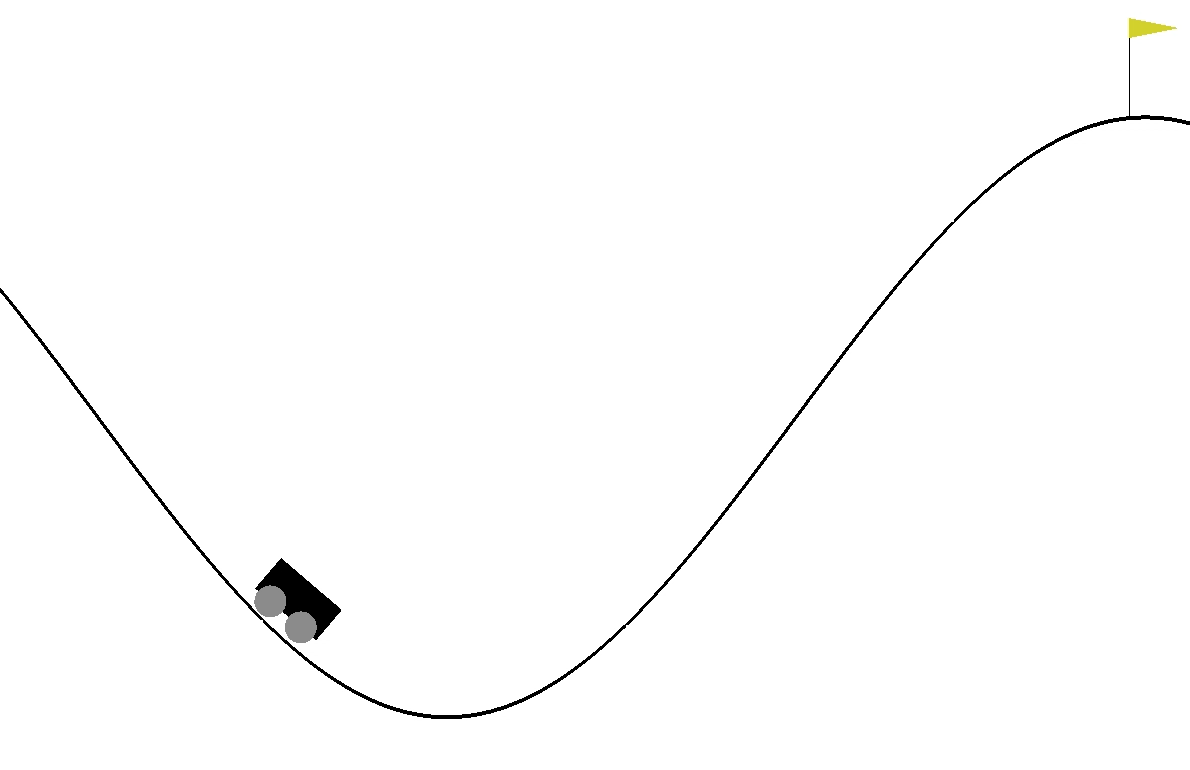
\includegraphics[width=4.8cm]{fig/lec10/mountain_car.png}
	\caption{Classic RL control example: mountain car (derivative work based on \href{https://github.com/openai/gym}{https://github.com/openai/gym}, MIT license)}
	\label{fig:Mountain_car_gym}
\end{figure}
\end{minipage}
\end{column}
\hfill
\begin{column}{0.54\textwidth}
\begin{minipage}[c]{\linewidth}
\begin{itemize}
	\item Two cont. states: position, velocity
	\item One discrete action: acceleration given by $\left\{\mbox{left},\mbox{none},\mbox{right}\right\}$ 
	\item $r_k=-1$, i.e., goal is to terminate episode as quick as possible
	\item Episode terminates when car reaches the flag (or max steps)
	\item Simplified longitudinal car physics with state constraints
	\item Position initialized randomly within valley, zero initial velocity
	\item Car is underpowered and requires swing-up
\end{itemize}
\end{minipage}
\end{column}
\end{columns}
}


%%%%%%%%%%%%%%%%%%%%%%%%%%%%%%%%%%%%%%%%%%%%%%%%%%%%%%%%%%%%%
%% Sarsa Application Example: Mountain Car (2)%%
%%%%%%%%%%%%%%%%%%%%%%%%%%%%%%%%%%%%%%%%%%%%%%%%%%%%%%%%%%%%%
\frame{\frametitle{SARSA application example: mountain car (2)}
\begin{figure}
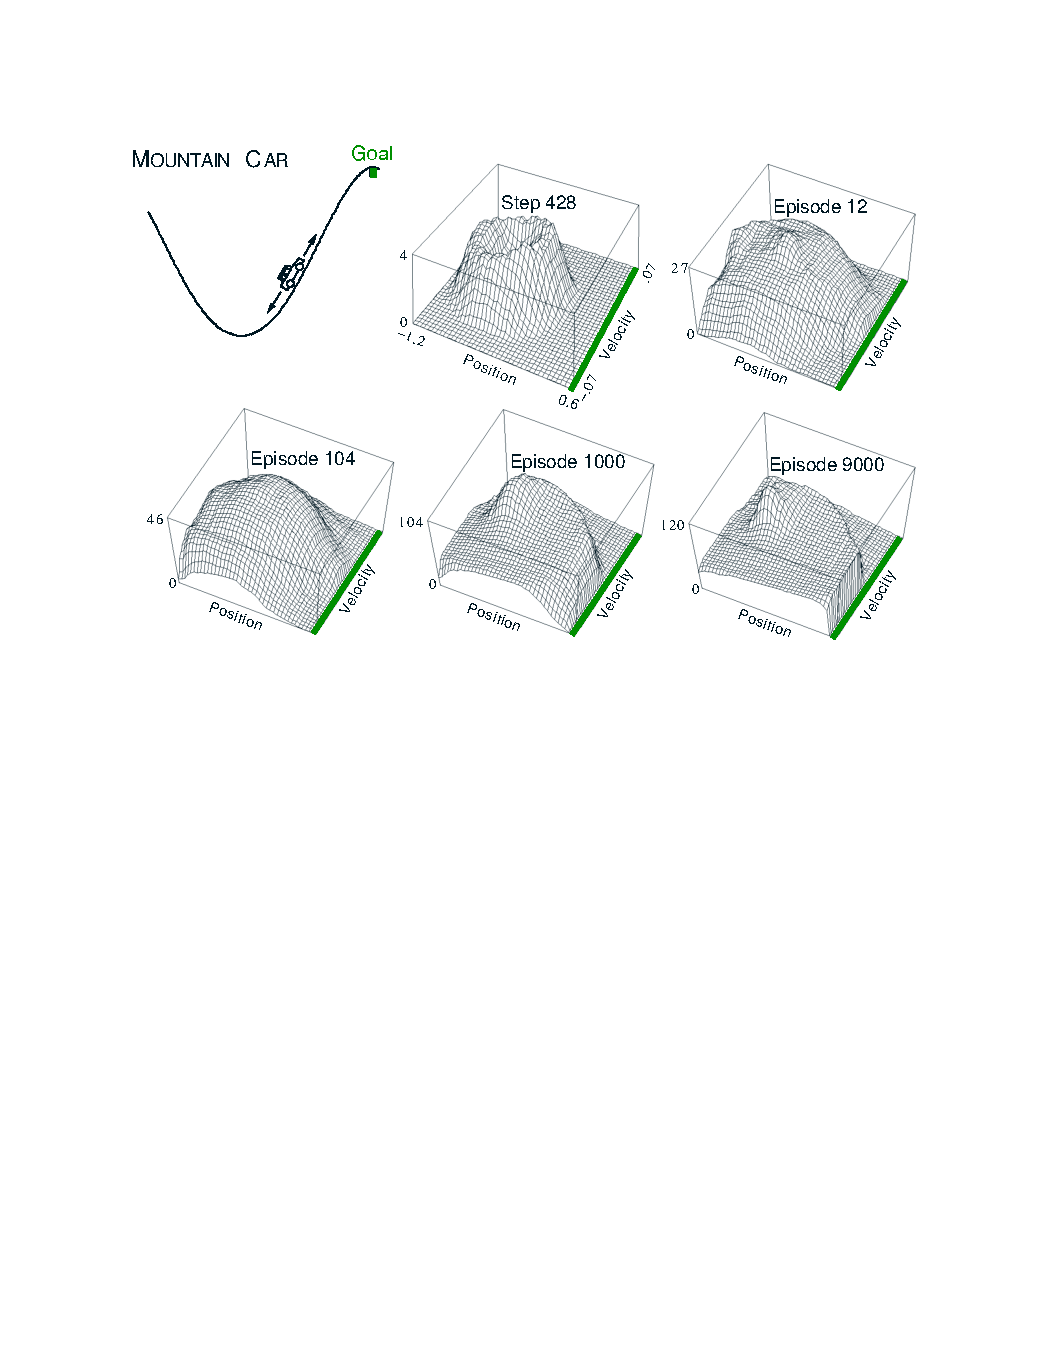
\includegraphics[height=0.65\textheight]{fig/lec10/Mountain_Car_BS.pdf}
\caption{Cost-to-go function $-\max_u \hat{q}(\bm{x},u,\bm{w})$ for mountain car task using linear approximation with SARSA and tile coding (source: R. Sutton and G. Barto, Reinforcement learning: an introduction, 2018, \href{https://creativecommons.org/licenses/by-nc-nd/2.0/}{CC BY-NC-ND 2.0})}
\end{figure}
}

%%%%%%%%%%%%%%%%%%%%%%%%%%%%%%%%%%%%%%%%%%%%%%%%%%%%%%%%%%%%%
%% Tile Coding %%
%%%%%%%%%%%%%%%%%%%%%%%%%%%%%%%%%%%%%%%%%%%%%%%%%%%%%%%%%%%%%
\frame{\frametitle{Tile coding}
\begin{itemize}
	\item Problem space is grouped into (overlapping) partitions / tiles.
	\item Performs a discretization of the problem space.
	\item Function approximation serves as interpolation between tiles.
	\item Find an example here: \href{https://github.com/MeepMoop/tilecoding}{https://github.com/MeepMoop/tilecoding} .
\end{itemize}
\begin{figure}
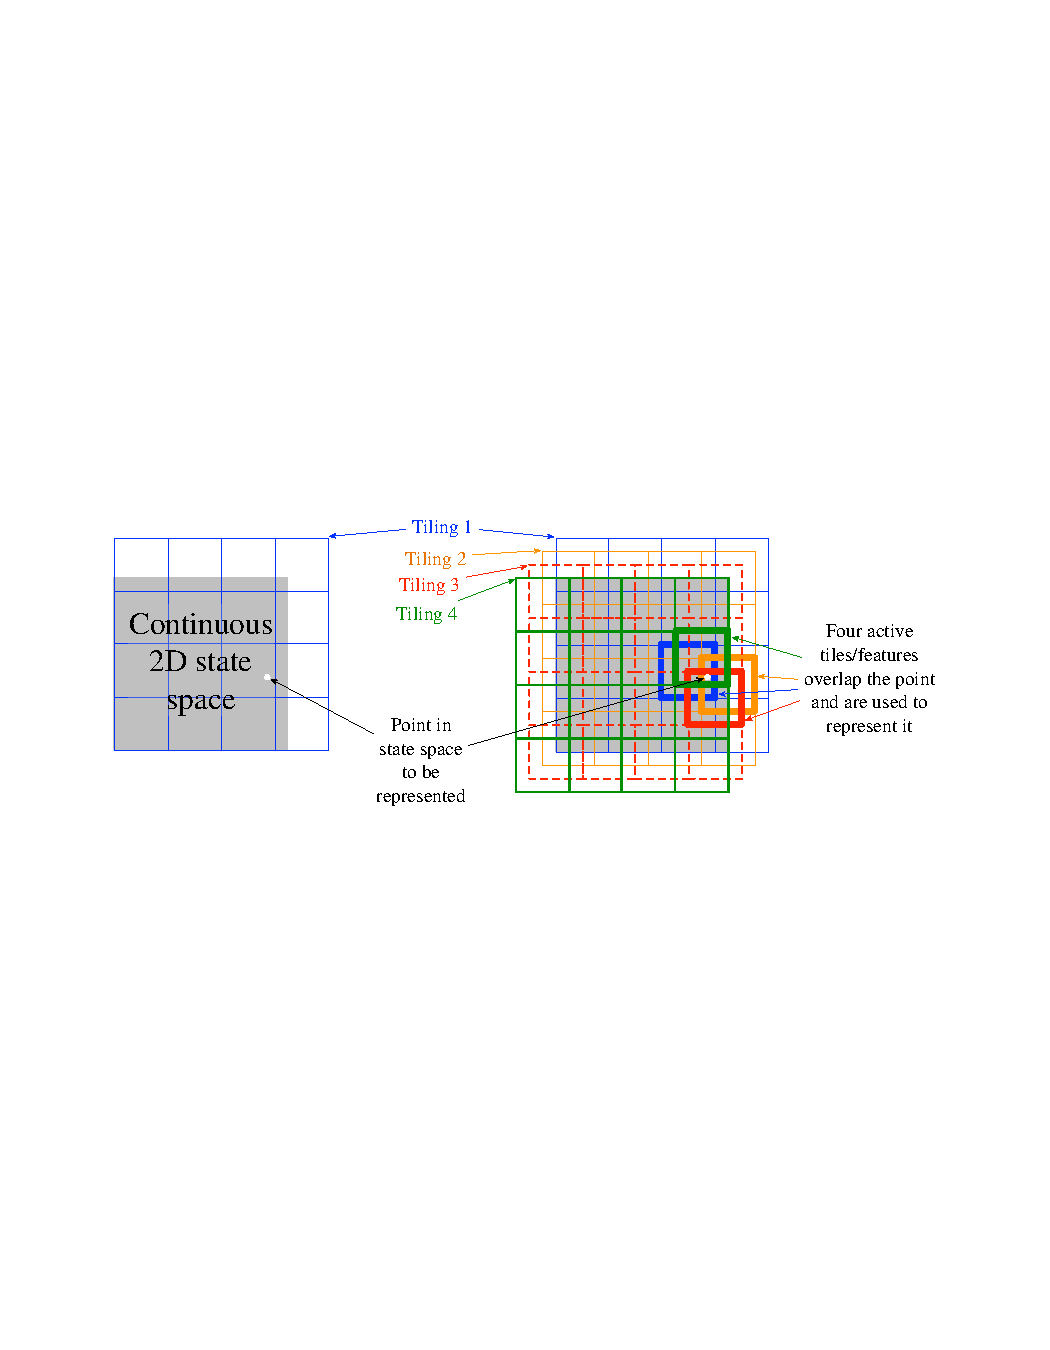
\includegraphics[width=10cm]{fig/lec10/Tile_Coding.pdf}
\caption{Tile coding example in 2D (source: R. Sutton and G. Barto, Reinforcement learning: an introduction, 2018, \href{https://creativecommons.org/licenses/by-nc-nd/2.0/}{CC BY-NC-ND 2.0})}
\end{figure}
}

%%%%%%%%%%%%%%%%%%%%%%%%%%%%%%%%%%%%%%%%%%%%%%%%%%%%%%%%%%%%%
%% n-step Semi-Gradient Sarsa %%
%%%%%%%%%%%%%%%%%%%%%%%%%%%%%%%%%%%%%%%%%%%%%%%%%%%%%%%%%%%%%
\frame{
\setlength{\algomargin}{0.5em}
\begin{algorithm}[H]
\footnotesize
\SetKwInput{Input}{input} 
\SetKwInput{Output}{output}
\SetKwInput{Init}{init}
\SetKwInput{Param}{parameter}
\Input{a differentiable function $\hat{q}:\mathbb{R}^\kappa\times\mathbb{R}^\zeta\rightarrow\mathbb{R}$}
\Input{a policy $\pi$ (only if estimating $q_\pi$)}
\Param{$\alpha\in\left\{\mathbb{R}|0<\alpha<1\right\}$, $\varepsilon\in\left\{\mathbb{R}|0<\varepsilon<<1\right\}$, $n\in\mathbb{Z}^+$}
\Init{parameter vector $\bm{w}\in\mathbb{R}^\zeta$ arbitrarily}
 \For{$j=1,2\ldots$ episodes}{
		initialize and store $\bm{x}_{0}$\;
		select and store $u_0\sim\pi(\bm{x}_0)$ or $\varepsilon$-greedy w.r.t. $\hat{q}(\bm{x}_0, \cdot, \bm{w})$\;
		$T\leftarrow\infty$\;
		\Repeat( $k=0, 1, 2, \ldots$){$\tau=T-1$}{
			\If{$k<T$}{
				take action $u_k$ observe and store $\bm{x}_{k+1}$ and $r_{k+1}$\;
				\lIf{$\bm{x}_{k+1}$ is terminal}{$T\leftarrow k+1$} \lElse{select \& store $u_{k+1}\sim\pi(\bm{x}_{k+1})$ or $\varepsilon$-greedy w.r.t. $\hat{q}(\bm{x}_{k+1}, \cdot, \bm{w})$}
				}
			$\tau\leftarrow k-n+1$ ($\tau$ time index for estimate update)\;
			\If{$\tau \geq 0$}{
				$g\leftarrow \sum_{i=\tau+1}^{\min(\tau + n, T)}\gamma^{i-\tau-1} r_i$\;
				if $\tau+n < T$: $g\leftarrow g + \gamma^n \hat{q}(\bm{x}_{\tau+n}, u_{\tau+n},\bm{w})$\;
				$\bm{w} \leftarrow \bm{w} + \alpha\left[g - \hat{q}(\bm{x}_\tau, u_\tau, \bm{w})\right]\nabla_{\bm{w}} \hat{q}(\bm{x}_\tau, u_\tau, , \bm{w})$\; 
			}
		}
	}
\caption{$n$-step semi-gradient SARSA (output: parameter vector $\bm{w}$ for $\hat{q}_\pi$ or $\hat{q}^*$)}
\label{algo:Semi_gradient_Sarsa_nstep}
\end{algorithm}
}

%%%%%%%%%%%%%%%%%%%%%%%%%%%%%%%%%%%%%%%%%%%%%%%%%%%%%%%%%%%%%%%%%%
\section{Least squares policy iteration (LSPI)} 
%%%%%%%%%%%%%%%%%%%%%%%%%%%%%%%%%%%%%%%%%%%%%%%%%%%%%%%%%%%%%%%%%%
\begin{frame}
\frametitle{Table of contents}
\tableofcontents[currentsection]
\end{frame}


%%%%%%%%%%%%%%%%%%%%%%%%%%%%%%%%%%%%%%%%%%%%%%%%%%%%%%%%%%%%%
%% Transfering LSTD-Style Batch Learning to Action Values %%
%%%%%%%%%%%%%%%%%%%%%%%%%%%%%%%%%%%%%%%%%%%%%%%%%%%%%%%%%%%%%
\frame{\frametitle{Transferring LSTD-style batch learning to action values}
\begin{itemize}
	\item In the previous lecture we developed a closed-form batch learning tool: LSTD.
	\begin{itemize}
		\item Linear function approximation.
		\item Fixed, representative data set $\bm{\mathcal{D}}$.
	\end{itemize}\pause
\item Same idea can be transferred to action values when bootstrapping with one-step Sarsa, called \hl{LS-SARSA} (or sometimes LSTD$Q$):
\begin{equation}
\begin{split}
	q_\pi(\bm{x}_k, u_k) &\approx r_{k+1}+\gamma\hat{q}(\bm{x}_{k+1}, u_{k+1}, \bm{w}_k),\\
	\hat{q}(\bm{x}_k, u_k, \bm{w}_k)&=\hat{q}(\tilde{\bm{x}}_k, \bm{w}_k)= \tilde{\bm{x}}\T_k\bm{w}_k .
\end{split}
\label{eq:bootstrapping_LSTDQ}
\end{equation}
\pause\vspace{-0.2cm} 
\item The cost function for action-value prediction is then:
\begin{equation}
	J(\bm{w}) = \sum_k \left[r_{k+1} - \left(\tilde{\bm{x}}\T_{k} - \gamma \tilde{\bm{x}}\T_{k+1}\right)\bm{w}\right]^2.
\end{equation}\pause\vspace{-0.2cm} 
\item Hence, the closed-form least squares solution for the action values is the same as for the state value case but the feature vector depends also on the actions:
\begin{equation*}
	\tilde{\bm{x}}_k = \bm{f}(\bm{x}_k, u_k).
\end{equation*}
\end{itemize}
}

%%%%%%%%%%%%%%%%%%%%%%%%%%%%%%%%%%%%%%%%%%%%%%%%%%%%%%%%%%%%%
%% On and Off-Policy LSTDQ %%
%%%%%%%%%%%%%%%%%%%%%%%%%%%%%%%%%%%%%%%%%%%%%%%%%%%%%%%%%%%%%
\frame{\frametitle{On and off-policy LS-SARSA}
With $b$ samples we can form a target vector $\bm{y}$ and regressor matrix $\bm{\Xi}$:
\begin{equation}
	\bm{y} = \begin{bmatrix} r_1 \\ r_2 \\ \vdots \\ r_b \end{bmatrix}, \quad \bm{\Xi}=\begin{bmatrix} \left(\tilde{\bm{x}}\T_{0} - \gamma \tilde{\bm{x}}\T_{1}\right) \\ \left(\tilde{\bm{x}}\T_{1} - \gamma \tilde{\bm{x}}\T_{2}\right)\\ \vdots \\\left(\tilde{\bm{x}}\T_{b-1} - \gamma \tilde{\bm{x}}\T_{b}\right) \end{bmatrix}\, .
	\label{eq:LSTDQ_data}
\end{equation}\pause
Regarding the data input to $\bm{\Xi}$ we can distinguish two cases: The actions $u_k$ and $u_{k+1}$ in the feature pair $\left(\tilde{\bm{x}}\T_{k} - \gamma \tilde{\bm{x}}\T_{k+1}\right)$ per row in $\bm{\Xi}$ either descends from the
\begin{itemize}
	\item \hl{same policy $\pi$ (on-policy learning)} or \pause
	\item the action $u_{k+1}$ in $\tilde{\bm{x}}_{k+1} = \bm{f}(\bm{x}_{k+1}, u_{k+1})$ is chosen based on an \hl{arbitrary policy $\pi'$ (off-policy learning)}. 
\end{itemize}\pause
If we apply off-policy LS-SARSA then
\begin{itemize}
	\item we retrieve the flexibility to collect training samples arbitrarily
	\item at the cost of an estimation bias based on the sampling distribution.
\end{itemize}
}

%%%%%%%%%%%%%%%%%%%%%%%%%%%%%%%%%%%%%%%%%%%%%%%%%%%%%%%%%%%%%
%% On and Off-Policy LSTDQ %%
%%%%%%%%%%%%%%%%%%%%%%%%%%%%%%%%%%%%%%%%%%%%%%%%%%%%%%%%%%%%%
\frame{\frametitle{LS-SARSA}
\begin{block}{LS-Sarsa solution}
Having arranged $i=1,\ldots,b$ samples $\left\langle \bm{x}_i, u_i, r_{i+1}, \bm{x}_{i+1}, u_{i+1}\right\rangle\sim\bm{\mathcal{D}}$ using one-step bootstrapping \eqref{eq:bootstrapping_LSTDQ} and linear function approximation as in \eqref{eq:LSTDQ_data}, the LS-SARSA solution is
\begin{equation}
		\bm{w}^* = (\bm{\Xi}\T\bm{\Xi})^{-1}\bm{\Xi}\T\bm{y} .
\end{equation}
\end{block}\pause
Again, basic usage distinction:
\begin{itemize}
	\item If $\left\{u_i, u_{i+1}\right\}\sim\pi$: on-policy prediction (as in LSTD)
	\item If $u_i\sim\pi$ and $u_{i+1}\sim\pi'$: off-policy prediction (useful for control) 
\end{itemize}\pause
Possible modifications:
\begin{itemize}
	\item To prevent numeric instability regularization is possible, cf. \eqref{eq:Ridge_LSTD}
	\item Recursive implementation for online usage straightforward, cf. \eqref{eq:RLS}
\end{itemize}
}

%%%%%%%%%%%%%%%%%%%%%%%%%%%%%%%%%%%%%%%%%%%%%%%%%%%%%%%%%%%%%
%% Least Squares Policy Iteration (LSPI) %%
%%%%%%%%%%%%%%%%%%%%%%%%%%%%%%%%%%%%%%%%%%%%%%%%%%%%%%%%%%%%%
\frame{\frametitle{Least squares policy iteration (LSPI)}
General idea:
\begin{itemize}
	\item Apply general policy improvement (GPI) based on data set $\bm{\mathcal{D}}$, 
	\item Policy evaluation by off-policy LS-SARSA,
	\item Policy improvement by greedy choices on predicted action values.
\end{itemize}
\begin{figure}
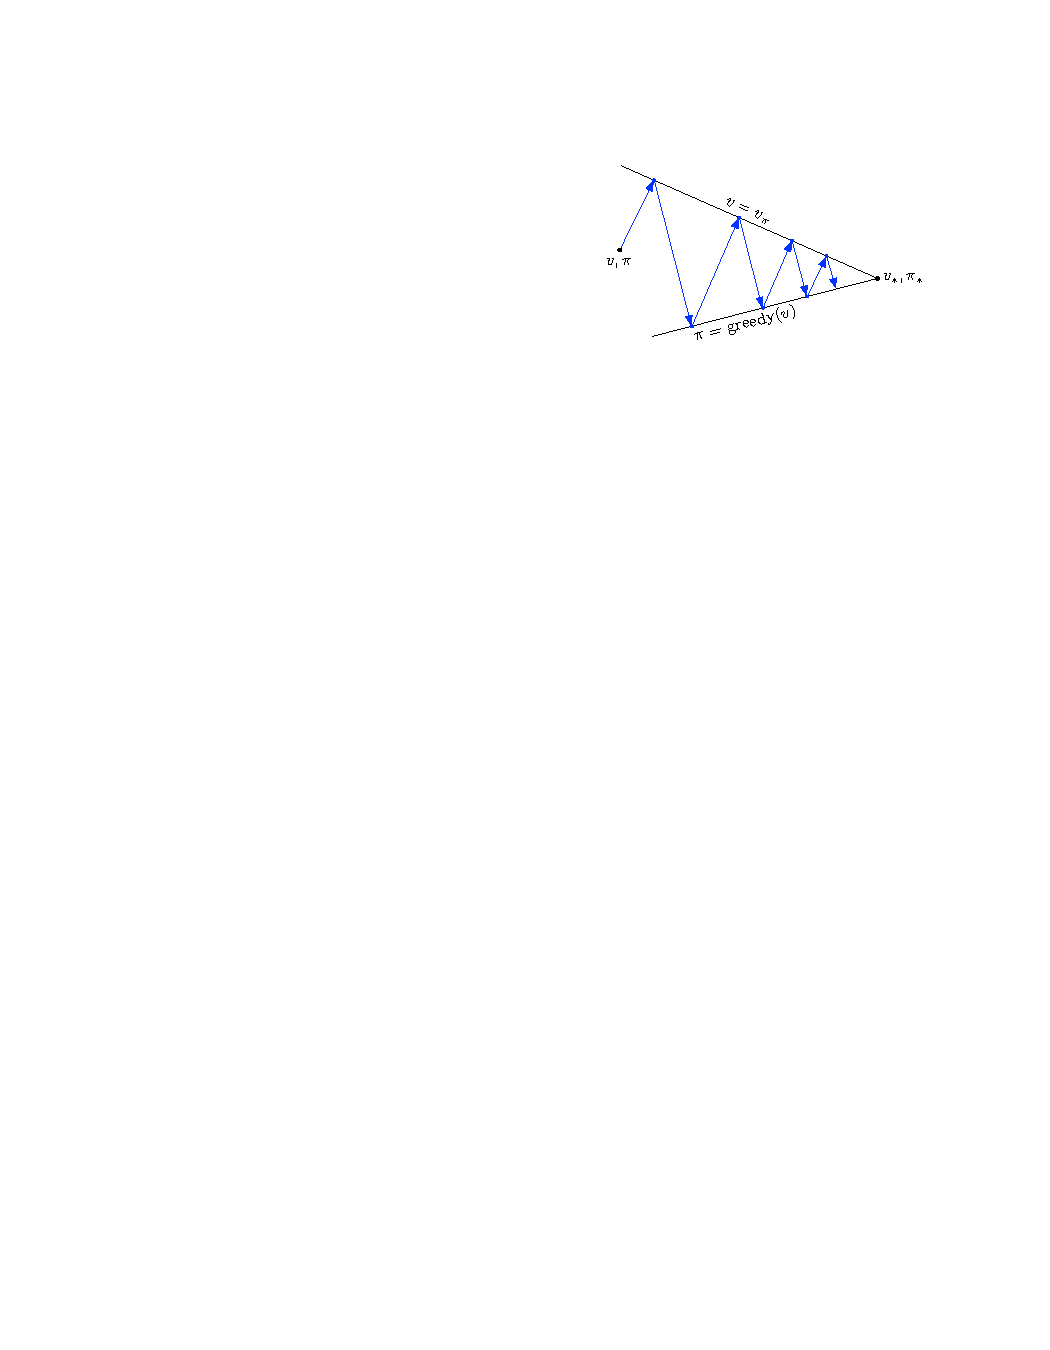
\includegraphics[height=0.3\textheight]{fig/lec03/GPI_02.pdf}
\end{figure}\pause
Some remarks:
\begin{itemize}
	\item LSPI is an offline and off-policy control approach.
	\item Exploration is required by feeding suitable sampling distributions in $\bm{\mathcal{D}}$:
	\begin{itemize}
		\item Such as $\varepsilon$-greedy choices based on $\hat{q}$. 
		\item But also complete random samples are conceivable.
	\end{itemize}
\end{itemize}
}


%%%%%%%%%%%%%%%%%%%%%%%%%%%%%%%%%%%%%%%%%%%%%%%%%%%%%%%%%%%%%
%% Semi-Gradient Sarsa %%
%%%%%%%%%%%%%%%%%%%%%%%%%%%%%%%%%%%%%%%%%%%%%%%%%%%%%%%%%%%%%
\frame{\frametitle{Algorithmic implementation: LSPI}
\setlength{\algomargin}{0.5em}
\begin{algorithm}[H]
\small
\SetKwInput{Input}{input} 
\SetKwInput{Output}{output}
\SetKwInput{Init}{init}
\SetKwInput{Param}{parameter}
\Input{a feature representation $\tilde{\bm{x}}$ with $\tilde{\bm{x}}_T=0$ (i.e., $\hat{q}(\tilde{\bm{x}}_T,\cdot)=0$)}
\Input{a data set $\left\langle \bm{x}_i, u_i, r_{i+1}, \bm{x}_{i+1}\right\rangle\sim\bm{\mathcal{D}}$ with $i=1,\ldots, b$ samples}
\Param{an accuracy threshold $\Delta\in\left\{\mathbb{R}|0<\Delta\right\}$}
\Init{linear approximation function weights $\bm{w}\in\mathbb{R}^\zeta$ arbitrarily}

$\pi\leftarrow \argmax_{u}\hat{q}(\cdot, u, \bm{w})$ (greedy choices based on $\hat{q}(\bm{w})$)\;
\Repeat{$||\bm{w}'-\bm{w}||<\Delta$}{
		$\bm{w}' \leftarrow \bm{w}$\;
		$\bm{w}\leftarrow\mbox{LS-SARSA}(\bm{\mathcal{D}}, u_{i+1}\sim\pi)$\;
		$\pi\leftarrow \argmax_{u}\hat{q}(\cdot, u, \bm{w})$\;
}
\caption{Least squares policy iteration (output: $\bm{w}$ for $\hat{q}^*$)}
\label{algo:LSPI}
\end{algorithm}\pause
\begin{itemize}
	\item In a (small) discrete action space the $\argmax_{u}$ operation is straightforward. \pause
	\item After one full LSPI evaluation the data set $\bm{\mathcal{D}}$ might be altered to include new data obtained based on the updated $\bm{w}$ vector. \pause
	\item Source: M. Lagoudakis and R. Parr, \textit{Least-Squares Policy Iteration}, Journal of Machine Learning Research 4, pp. 1107-1149, 2003
\end{itemize}
}

%%%%%%%%%%%%%%%%%%%%%%%%%%%%%%%%%%%%%%%%%%%%%%%%%%%%%%%%%%%%%
%% LSPI Application Example: Inverted Pendulum %%
%%%%%%%%%%%%%%%%%%%%%%%%%%%%%%%%%%%%%%%%%%%%%%%%%%%%%%%%%%%%%
\frame{\frametitle{LSPI application example: inverted pendulum (1)}
\begin{columns}[t,onlytextwidth]
\begin{column}{0.475\textwidth}
\begin{minipage}[c]{\linewidth}
\begin{figure}
	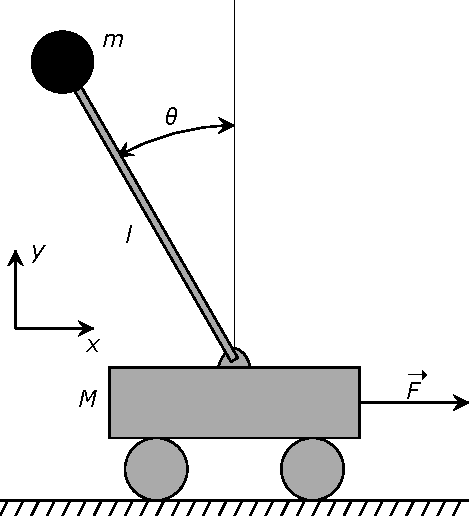
\includegraphics[width=4.8cm]{fig/lec10/Inv_pendulum.pdf}
	\caption{Classic RL control example: inverted pendulum (source: \href{https://commons.wikimedia.org/wiki/File:Cart-pendulum.svg}{www.wikipedia.org}, \href{https://creativecommons.org/publicdomain/zero/1.0/deed.en}{CC0 1.0})}
	\label{fig:Inv_pendulum}
\end{figure}
\end{minipage}
\end{column}
\hfill
\begin{column}{0.54\textwidth}
\begin{minipage}[c]{\linewidth}
\begin{itemize}
	\item Two continuous states: angular position $\theta$ and velocity $\dot{\theta}$
	\item One discrete action: acceleration force (i.e., torque at shaft)
	\item Action noise as disturbance 
	\item Non-linear system dynamics
	\item State initialization randomly close to upper equilibrium
	\item $r_k=0$ if pendulum is above horizontal line
	\item $r_k=-1$ if below horizontal line and episode terminates
	\item $\gamma=0.95$
\end{itemize}
\end{minipage}
\end{column}
\end{columns}
}

%%%%%%%%%%%%%%%%%%%%%%%%%%%%%%%%%%%%%%%%%%%%%%%%%%%%%%%%%%%%%
%% LSPI Application Example: Inverted Pendulum (2) %%
%%%%%%%%%%%%%%%%%%%%%%%%%%%%%%%%%%%%%%%%%%%%%%%%%%%%%%%%%%%%%
\frame{\frametitle{LSPI application example: inverted pendulum (2)}
\begin{itemize}
	\item Initial training samples for $\bm{\mathcal{D}}$ following a policy selecting actions at uniform probability
	\item Additional samples have been manually added during the training
	\item Radial basis function as feature engineering
\end{itemize}
\begin{figure}
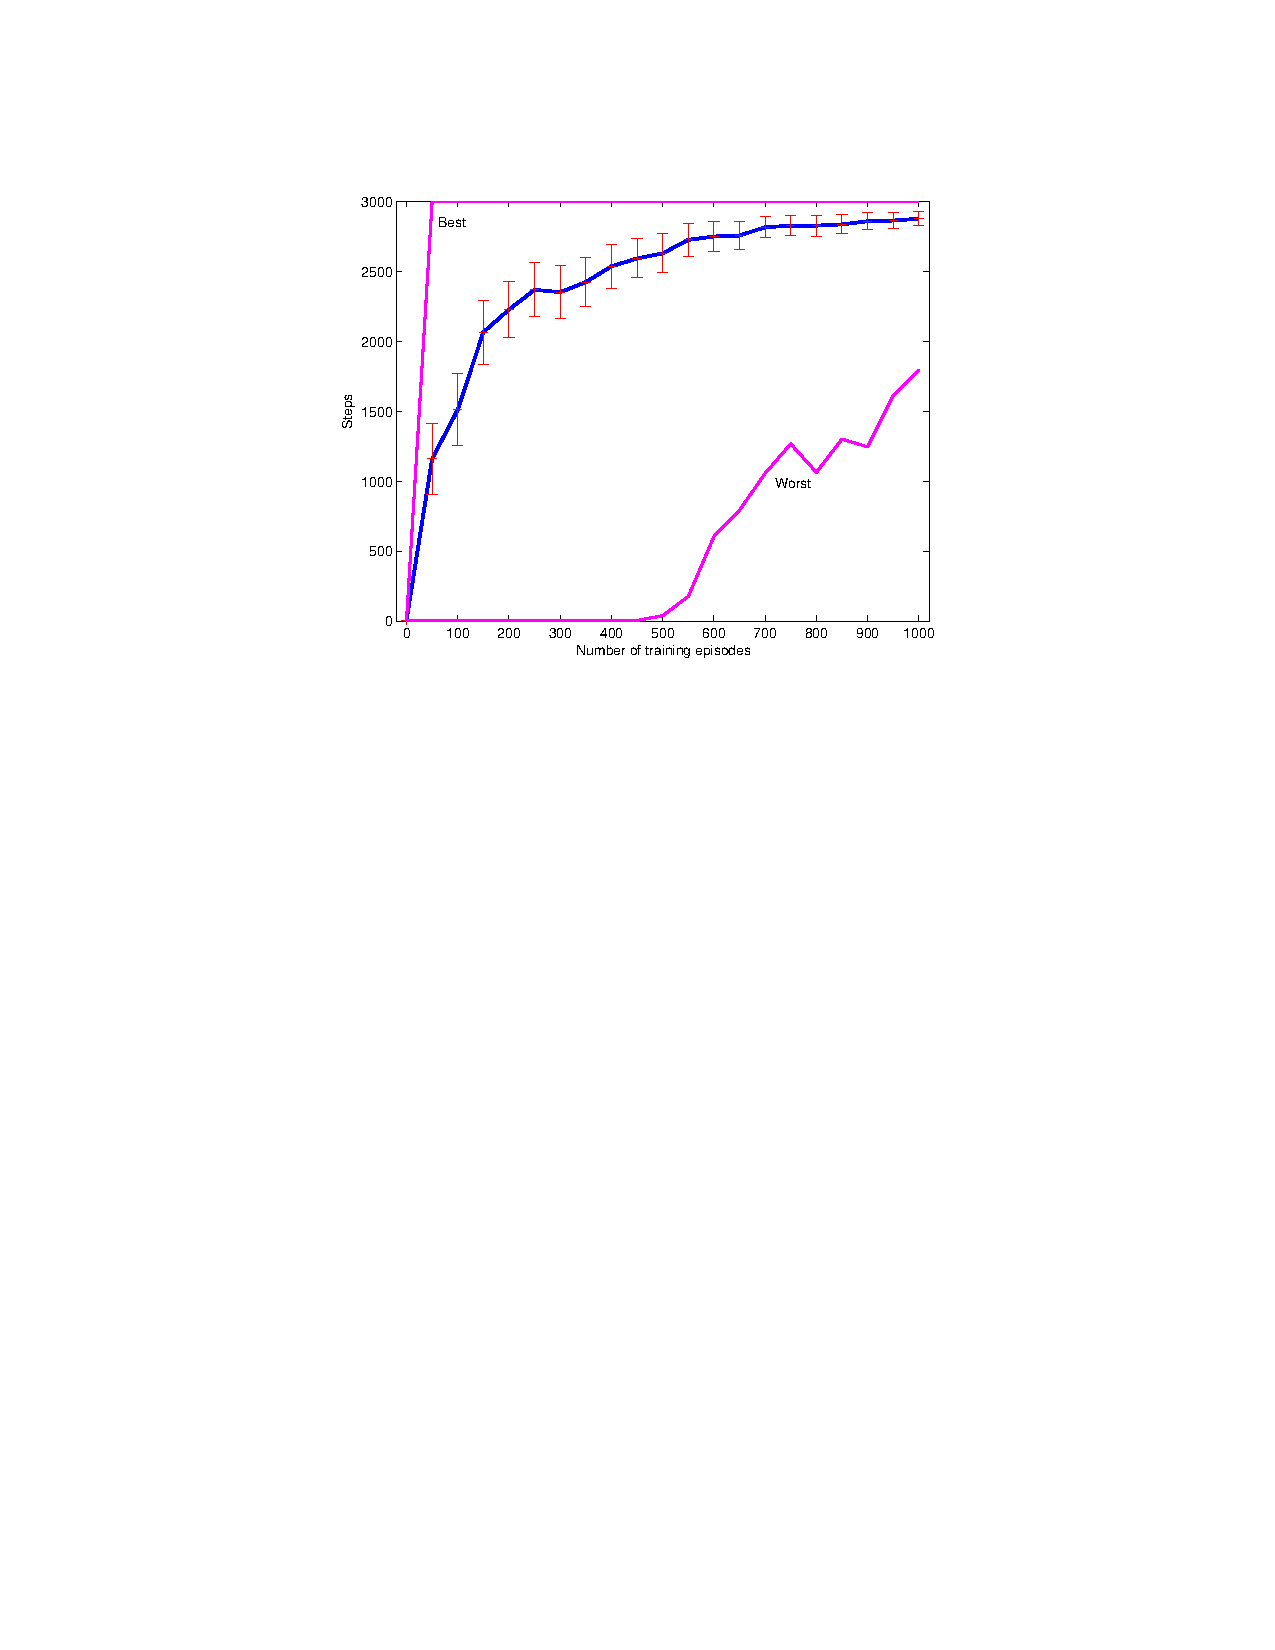
\includegraphics[height=4.2cm]{fig/lec10/LSPI_Inv_Pendulum.pdf}
\caption{Balancing steps before episode termination with a clipping of maximum 3000 steps (source: M. Lagoudakis and R. Parr, \textit{Least-Squares Policy Iteration}, Journal of Machine Learning Research 4, pp. 1107-1149, 2003)}
\end{figure}
}

%%%%%%%%%%%%%%%%%%%%%%%%%%%%%%%%%%%%%%%%%%%%%%%%%%%%%%%%%%%%%
%% RLS-TD Algorithmic Implementation  %%
%%%%%%%%%%%%%%%%%%%%%%%%%%%%%%%%%%%%%%%%%%%%%%%%%%%%%%%%%%%%%
\frame{\frametitle{Algorithmic implementation: online LSPI}
\setlength{\algomargin}{0.5em}
\vspace{-0.15cm}
\begin{algorithm}[H]
\small
\SetKwInput{Input}{input} 
\SetKwInput{Output}{output}
\SetKwInput{Init}{init}
\SetKwInput{Param}{parameter}
\Input{a feature representation $\tilde{\bm{x}}$ with $\tilde{\bm{x}}_T=0$ (i.e., $\hat{q}(\tilde{\bm{x}}_T,\cdot, \cdot)=0$)}
\Param{forgetting factor $\lambda\in\left\{\mathbb{R}|0 < \lambda \leq 1\right\}$, $\varepsilon\in\left\{\mathbb{R}|0<\varepsilon<<1\right\}$, update factor $k_w\in\left\{\mathbb{N}|1\leq k_w\right\}$}
\Init{weights $\bm{w}\in\mathbb{R}^\zeta$ arbitrarily, policy $\pi$ being $\varepsilon$-greedy w.r.t. $\hat{q}(\bm{w})$, covariance $\bm{P}>0$}
 \For{$j=1,2,\ldots$ episodes}{
		initialize $\bm{x}_{0}$ and set $u_0\sim\pi(\bm{x}_{0})$\;
		\For{$k=0, 1, 2 \ldots $ time steps}{
			apply action $u_k$, observe $\bm{x}_{k+1}$ and $r_{k+1}$, set $u_{k+1}\sim\pi(\bm{x}_{k+1})$\;
			$y \leftarrow r_{k+1}$\;
			$\bm{\xi}\T \leftarrow \tilde{\bm{x}}\T_{k}(\bm{x}_k, u_k) - \gamma \tilde{\bm{x}}\T_{k+1}(\bm{x}_{k+1}, u_{k+1})$\;
			$\bm{c} \leftarrow \left(\bm{P}\bm{\xi}\right)/\left(\lambda+\bm{\xi}\T\bm{P}\bm{\xi}\right)$\;
			$\bm{w} \leftarrow \bm{w} + \bm{c}\left(y-\bm{\xi}\T \bm{w}\right)$\;
			$\bm{P} \leftarrow \left(\bm{I} - \bm{c}\bm{\xi}\T\right)\bm{P}/\lambda$\;
			\If{$k \mod k_w=0$}{
					$\pi\leftarrow \varepsilon$-greedy w.r.t. $\hat{q}=\tilde{\bm{x}}\T(\bm{x},u)\bm{w}$\;
			}
			exit loop if $\bm{x}_{k+1}$ is terminal\;
		}
	}
\caption{Online LSPI with RLS-SARSA (output: $\bm{w}$ for $\hat{q}^*$)}
\label{algo:LSPI_Online}
\end{algorithm}
}

%%%%%%%%%%%%%%%%%%%%%%%%%%%%%%%%%%%%%%%%%%%%%%%%%%%%%%%%%%%%%
%% Remarks on Online LSPI %%
%%%%%%%%%%%%%%%%%%%%%%%%%%%%%%%%%%%%%%%%%%%%%%%%%%%%%%%%%%%%%
\frame{\frametitle{Remarks on online LSPI}
\begin{itemize}
	\item $k_w$ depicts the number of steps between policy improvement cycles.\pause
	\item Forgetting factor $\lambda$ and $k_w$ require mutual tuning:
	\begin{itemize}
		\item After each policy improvement the policy evaluation requires sample updates to accurately predict the altered policy.
		\item Numerically instability may occur for $\lambda < 1$ and requires regularization.
	\end{itemize}\pause
	\item Hence, the algorithm is online-capable but its policy is normally not updated in a step-by-step fashion.\pause
	\item Alternative online LSPI with OLS-SARSA can be found in L.~Bu{\c{s}}oniu~et~al., \textit{Online least-squares policy iteration for reinforcement learning control}, American Control Conference, 2010.
\end{itemize}
}

%%%%%%%%%%%%%%%%%%%%%%%%%%%%%%%%%%%%%%%%%%%%%%%%%%%%%%%%%%%%%%%%%%
\section{Deep \texorpdfstring{$q$}{Q}-networks (DQN)} 
%%%%%%%%%%%%%%%%%%%%%%%%%%%%%%%%%%%%%%%%%%%%%%%%%%%%%%%%%%%%%%%%%%
\begin{frame}
\frametitle{Table of contents}
\tableofcontents[currentsection]
\end{frame}

%%%%%%%%%%%%%%%%%%%%%%%%%%%%%%%%%%%%%%%%%%%%%%%%%%%%%%%%%%%%%
%% General Background on DQN  %%
%%%%%%%%%%%%%%%%%%%%%%%%%%%%%%%%%%%%%%%%%%%%%%%%%%%%%%%%%%%%%
\frame{\frametitle{General background on DQN}
\begin{itemize}
	\item Recall incremental learning step from tabular $Q$-learning:
	\begin{equation*}
		\hat{q}(x, u) \leftarrow \hat{q}(x, u) + \alpha\left[r+\gamma \max_u \hat{q}(x', u) - \hat{q}(x, u)\right] .
		\end{equation*}\pause
	\item \hl{Deep $Q$-networks (DQN)}	transfer this to an approximate solution:
	\end{itemize}
	 \begin{equation}
	 \bm{w} = \bm{w} + \alpha\left[r+\gamma \max_u \hat{q}(\bm{x}', u, \bm{w}) - \hat{q}(\bm{x}, u, \bm{w})\right]\nabla_{\bm{w}} \hat{q}(\bm{x}, u, \bm{w}).
 \end{equation}\pause
However, instead of using above semi-gradient step-by-step updates, DQN is characterized by
	\begin{itemize}
		\item an \hl{experience replay buffer} for batch learning (cf. prev. lectures),\pause
		\item a separate set of \hl{weights $\bm{w}^-$ for the bootstrapped $Q$-target}. 
	\end{itemize}\pause
Motivation behind:
\begin{itemize}
	\item Efficiently use available data (experience replay).
	\item Stabilize learning by trying to make targets and feature inputs more like i.i.d. data from a stationary process (prevent windup of values). 
\end{itemize}
}

%%%%%%%%%%%%%%%%%%%%%%%%%%%%%%%%%%%%%%%%%%%%%%%%%%%%%%%%%%%%%
%% Summary of DQN Working Principle  (1)%%
%%%%%%%%%%%%%%%%%%%%%%%%%%%%%%%%%%%%%%%%%%%%%%%%%%%%%%%%%%%%%
\frame{\frametitle{Summary of DQN working principle (1)}
\begin{itemize}
	\item Take actions $u$ based on $\hat{q}(\bm{x},u,\bm{w})$ (e.g., $\varepsilon$-greedy). \pause
	\item Store observed tuples $\left\langle \bm{x}, u, r, \bm{x}'\right\rangle$ in memory buffer $\bm{\mathcal{D}}$.\pause
	\item Sample mini-batches $\bm{\mathcal{D}}_b$ from $\bm{\mathcal{D}}$. 
	\item Calculate bootstrapped $Q$-target with a delayed parameter vector $\bm{w}^-$ (so-called target network):
	\begin{equation*}
		 q_\pi(\bm{x},u)\approx r+\gamma \max_u \hat{q}(\bm{x}',u,\bm{w}^-).
	\end{equation*}\pause
	\item Optimize MSE loss between above targets and the regular approximation $\hat{q}(\bm{x},u,\bm{w})$ using $\bm{\mathcal{D}}_b$
	\begin{equation}
				\mathcal{L}(\bm{w}) = \left[\left(r+ \gamma \max_u \hat{q}(\bm{x}',u,\bm{w}^-)\right) - \hat{q}(\bm{x},u,\bm{w}) \right]^2_{\bm{\mathcal{D}}_b} \, .
	\end{equation}\pause
	\item Update $\bm{w}^-$ based on $\bm{w}$ from time to time.
 \end{itemize}
}

%%%%%%%%%%%%%%%%%%%%%%%%%%%%%%%%%%%%%%%%%%%%%%%%%%%%%%%%%%%%%
%% Summary of DQN Working Principle  (2)%%
%%%%%%%%%%%%%%%%%%%%%%%%%%%%%%%%%%%%%%%%%%%%%%%%%%%%%%%%%%%%%
\frame{\frametitle{Summary of DQN working principle (2)}
\begin{figure}
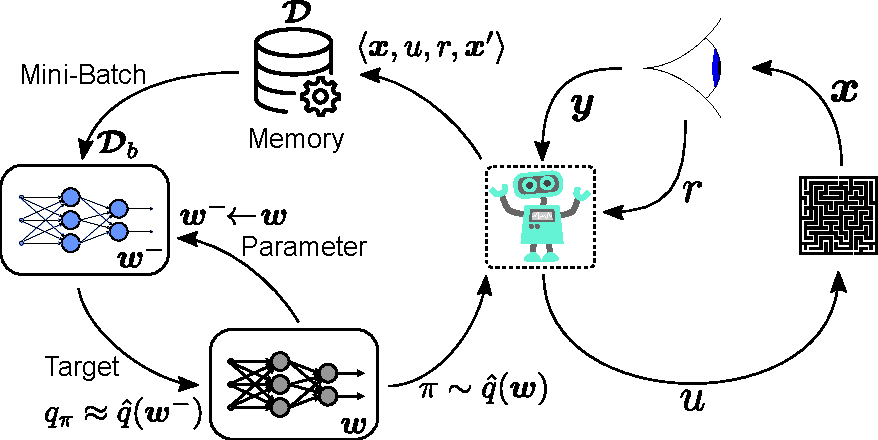
\includegraphics[height=5.5cm]{fig/lec10/DQN.pdf}
\caption{DQN structure from a bird's-eye perspective (derivative work of \figref{fig:RL_Wiki} and \href{https://commons.wikimedia.org/wiki/File:Multi-Layer_Neural_Network-Vector.svg?uselang=de}{wikipedia.org}, \href{https://creativecommons.org/publicdomain/zero/1.0/deed.en}{CC0 1.0})}
\label{fig:DQN}
\end{figure}
}		

%%%%%%%%%%%%%%%%%%%%%%%%%%%%%%%%%%%%%%%%%%%%%%%%%%%%%%%%%%%%%
%% Algo DQN %%
%%%%%%%%%%%%%%%%%%%%%%%%%%%%%%%%%%%%%%%%%%%%%%%%%%%%%%%%%%%%%
\frame{\frametitle{Algorithmic implementation: DQN}
\setlength{\algomargin}{0.5em}
\begin{algorithm}[H]
\small
\SetKwInput{Input}{input} 
\SetKwInput{Output}{output}
\SetKwInput{Init}{init}
\SetKwInput{Param}{parameter}
\Input{a differentiable function $\hat{q}:\mathbb{R}^\kappa\times\mathbb{R}^\zeta\rightarrow\mathbb{R}$ (including feature eng.)}
\Param{$\varepsilon\in\left\{\mathbb{R}|0<\varepsilon<<1\right\}$, update factor $k_w\in\left\{\mathbb{N}|1\leq k_w\right\}$}
\Init{weights $\bm{w}=\bm{w}^-\in\mathbb{R}^\zeta$ arbitrarily, memory $\bm{\mathcal{D}}$ with certain capacity}
 \For{$j=1,2,\ldots$ episodes}{
		initialize $\bm{x}_{0}$\;
		\For{$k=0, 1, 2 \ldots $ time steps}{
			$u_k \leftarrow$ apply action $\varepsilon$-greedy w.r.t $\hat{q}(\bm{x}_k, \cdot, \bm{w})$\;
			observe $\bm{x}_{k+1}$ and $r_{k+1}$\;
			store tuple $\left\langle \bm{x}_k, u_k, r_{k+1}, \bm{x}_{k+1}\right\rangle$ in $\bm{\mathcal{D}}$\;
			sample mini-batch $\bm{\mathcal{D}}_b$ from $\bm{\mathcal{D}}$ (after initial memory warmup)\;
			\For(calculate $Q$-targets){$i=1,\ldots,b$ samples}{
				\lIf{$\bm{x}_{i+1}$ is terminal}{$y_i=r_{i+1}$}
				\lElse{$y_i= r_{i+1}+ \gamma \max_u \hat{q}(\bm{x}_{i+1},u,\bm{w}^-)$}
			}
			fit $\bm{w}$ on loss $\mathcal{L}(\bm{w})=[y_i - \hat{q}(\bm{x}_i, u_i, \bm{w})]^2_{\bm{\mathcal{D}}_b}$\;
			\lIf{$k \mod k_w=0$}{$\bm{w}^-\leftarrow \bm{w}$ (update target weights)}
			}
}
\caption{DQN (output: parameter vector $\bm{w}$ for $\hat{q}^*$)}
\label{algo:DQN}
\end{algorithm}
}

%%%%%%%%%%%%%%%%%%%%%%%%%%%%%%%%%%%%%%%%%%%%%%%%%%%%%%%%%%%%%
%% Remarks on DQN Implementation %%
%%%%%%%%%%%%%%%%%%%%%%%%%%%%%%%%%%%%%%%%%%%%%%%%%%%%%%%%%%%%%
\frame{\frametitle{Remarks on DQN implementation}
\begin{itemize}
	\item General framework is based on V. Mnih et al., \textit{Human-level control through deep reinforcement learning}, Nature, pp. 529-533, 2015.\pause
	\item Often 'deep' artificial neural networks are used as function approximation for DQN.
	\begin{itemize}
		\item Nevertheless, other model topologies are fully conceivable.\pause
	\end{itemize}
	\item The fit of $\bm{w}$ on loss $\mathcal{L}$ is an intermediate supervised learning step.
	\begin{itemize}
		\item Comes with degrees of freedom regarding solver choice.
		\item Has own optimization parameters which are not depicted here in details (many tuning options).
	\end{itemize}\pause
	\item Mini-batch sampling from $\bm{\mathcal{D}}$ is often randomly distributed.
		\begin{itemize}
		\item Nevertheless, guided sampling with useful distributions for a specific control task can be beneficial (cf. Dyna discussion in 7th lecture).
	\end{itemize}\pause
	\item Likewise, the simple $\varepsilon$-greedy approach can be extended.
	\begin{itemize}
		\item Often a scheduled/annealed trajectory $\varepsilon_k$ is used.
		\item Again referring to the Dyna framework, many more exploration strategies are possible. 
	\end{itemize}
 \end{itemize}
}


%%%%%%%%%%%%%%%%%%%%%%%%%%%%%%%%%%%%%%%%%%%%%%%%%%%%%%%%%%%%%
%% DQN Application Example: Atari Games (1) %%
%%%%%%%%%%%%%%%%%%%%%%%%%%%%%%%%%%%%%%%%%%%%%%%%%%%%%%%%%%%%%
\frame{\frametitle{DQN application example: Atari games (1)}
\begin{itemize}
	\item End-to-end learning of $\hat{q}(\bm{x},u)$ from monitor pixels $\bm{x}$
	\item Feature engineering obtains stacking of raw pixes from last 4 frames
	\item Actions $u$ are 18 possible joystick/button combinations
	\item Reward is the change of highscore per step
	\item Interesting lecture from V. Minh with more details: \href{https://www.youtube.com/watch?v=fevMOp5TDQs&t=1499s}{YouTube}
\end{itemize}
\begin{figure}
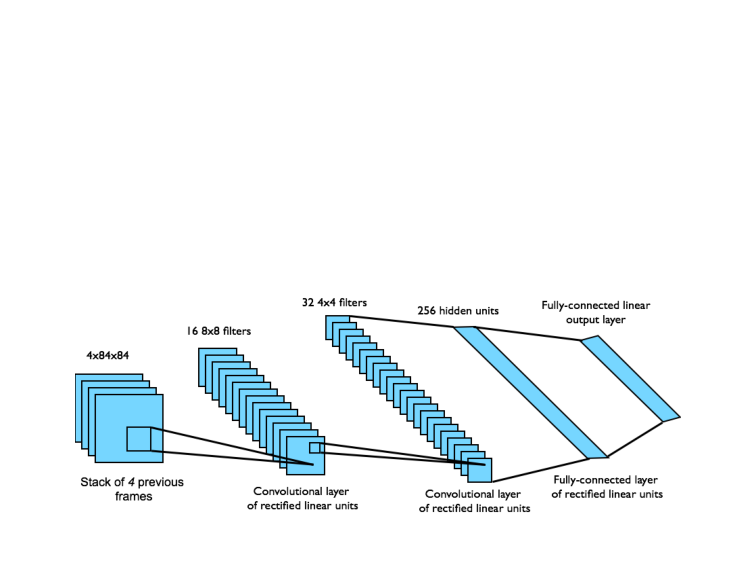
\includegraphics[height=0.4\textheight]{fig/lec10/DQN_Network_Silver.pdf}
\caption{Network architecture overview used for DQN in Atari games \SilverLectureSource}
\end{figure}
}

%%%%%%%%%%%%%%%%%%%%%%%%%%%%%%%%%%%%%%%%%%%%%%%%%%%%%%%%%%%%%
%% DQN Application Example: Atari Games (2%%%%%%%%%%%%%%%%%%%
\frame{\frametitle{DQN application example: Atari games (2)}
\begin{figure}
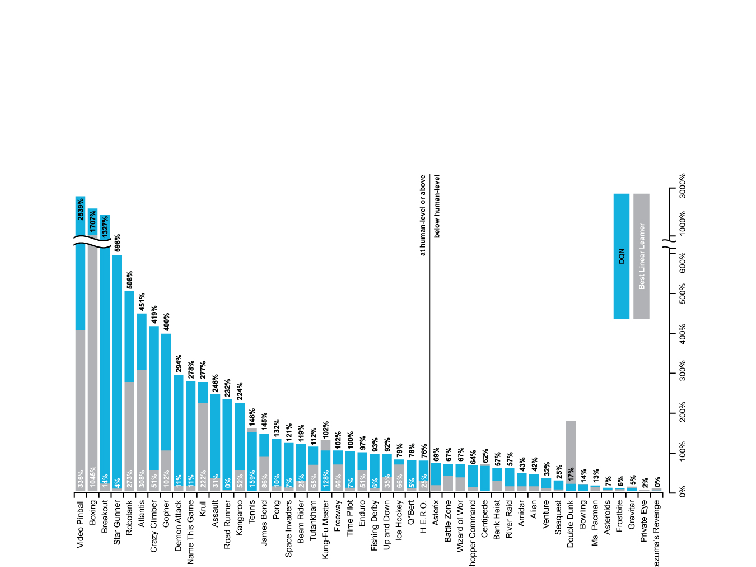
\includegraphics[height=0.7\textheight]{fig/lec10/DQN_Atari_Results.pdf}
\caption{DQN performance results in Atari games against human performance \SilverLectureSource}
\end{figure}
}

%%%%%%%%%%%%%%%%%%%%%%%%%%%%%%%%%%%%%%%%%%%%%%%%%%%%%%%%%%%%%
%% Summary %%
%%%%%%%%%%%%%%%%%%%%%%%%%%%%%%%%%%%%%%%%%%%%%%%%%%%%%%%%%%%%%
\begin{frame}
\frametitle{Summary: what you've learned today}
\begin{itemize}
	\item From a simplified perspective, the procedures from the approximate prediction can simply be transferred to value-based control.\pause
	\item On the contrary, the policy improvement theorem no longer applies in the approximate RL case (generalization impact).\pause
	\begin{itemize}
		\item Control algorithms may diverge completely.\pause
		\item Or a performance trade-off between different parts of the problem space could emerge.\pause
	\end{itemize}
	\item Off-policy batch learning approaches allow for efficient data usage.
	\begin{itemize}
		\item LSPI uses LS-SARSA on linear function approximation.\pause
		\item DQN extends $Q$-learning on non-linear approximation with additional tweaks (experience replay, target networks,...).\pause
		\item However, a prediction bias results (off-policy sampling distribution).  
	\end{itemize}
\end{itemize}
\end{frame}